\documentclass[twocolumn, english]{revtex4-2}
\usepackage{amsmath}
\usepackage{braket}
\usepackage{titlesec}
\usepackage{graphicx}
\usepackage{hyperref}
\graphicspath{ {./images/} }
\begin{document}

\title{Quantum unsupervised learning on a superconducting processor}
\author{Rupak Chatterjee}
\email{Rupak.Chatterjee@stevens.edu}
\author{Abhijat Sarma}
\email{absarma@ctemc.org}
\author{Ting Yu}
\email{ting.yu@stevens.edu}
\affiliation{Center for Quantum Science and Engineering\\
Department of Physics, Stevens Institute of Technology, Castle Point on the Hudson, Hoboken, NJ 07030}
\begin{abstract}
Various machine learning algorithms, namely K-means clustering and Support Vector Machines (SVMs), perform well on classifying and identifying patterns in wide ranges of datasets due to their versatility. However, as one increases the amount of data points and features, the computation time for training and using these statistical models grows intractably. The ability to store information compactly in quantum states suggests that quantum computers can be used to optimize such algorithms. Here, we propose and experimentally implement on superconducting qubits a quantum analogue to K-means clustering, and compare it to a previously developed quantum SVM. We apply the algorithm to the standard Wine and Iris datasets, and find that our quantum clustering algorithm can produce linear boundaries to a high degree of accuracy reflecting the true boundaries in the data.
\end{abstract}
\maketitle

\section{Introduction}
Machine learning offers solutions to several classes of problems unreachable through conventional computing means. For example, solutions to classification problems and regression of large datasets based on machine learning techniques are in general much more powerful than previously available solutions. These algorithms suffer in that they grow polynomially with the size and dimension of the data, which leads to substantial run times when dealing with large datasets, coined "big data". The ability of data to be more efficiently stored and manipulated in quantum states has recently lead to the proposal of several quantum algorithms for machine learning \cite{var_circ1, var_circ2, qml, autoencoders, feedforward, featureHilbertSpace, circuitcentric, lloydqsvm}. Building upon \cite{lloydlearning} and \cite{qmeans}, in this paper, we develop a hybrid \textit{K}-means clustering algorithm in order to identify clusters in data more quickly than possible with similar purely classical algorithms. The algorithm relies on a distance measure, here taken to be Euclidean square distance. This distance can be calculated efficiently on a quantum computer, as we will show, in order to speed up the algorithm as a whole. We compare our quantum K-means clustering algorithm to a classical one, in terms of accuracy in solving trinary classification problems on a real dataset. Additionally, we include a multiclass extension of the quantum SVM introduced in \cite{qsvm} in order to better understand differences between different quantum machine learning algorithms.

\section{Hybrid \textit{K}-means Clustering}

In machine learning theory, it is often mathematically convenient to consider the data as encoded in a vector. Therefore, each data point with \textit{P} different variables (features), can be encoded as a \textit{P}-dimensional feature vector. The total dataset is therefore a set of vectors in \textit{P}-dimensional space, known as input space. \textit{K}-means clustering is an unsupervised learning algorithm which considers the problem of partitioning \textit{N} feature vectors $\textbf{X}^{i}$ into \textit{K} \textit{subsets}, or \textit{clusters}. The algorithm seeks to find the \textit{K} clusters which minimize the dissimilarity between each cluster's members. Local minimization can be iteratively found with Lloyd's Algorithm, which relies on a distance measure, usually taken to be Euclidean square distance. 

Sampling and estimating Euclidean distances between post-processed vectors on a classical computer is known to be exponentially hard. For big data sets, the algorithm becomes slow as convergence relies on repeated calculations of this distance measure. In the next section, we propose and implement a quantum algorithm for calculating the Euclidean distance, which can be shown to be faster than the classical counterpart \cite{lloydlearning}. Note that although we use Euclidean distance in our clustering algorithm, one could use any distance measure. The Euclidean distance is desirable for our purposes because it assigns linear boundaries between clusters, and is guaranteed to converge, assuming no error in calculation (INSERT CITATION). For non-linear boundaries, one could use a corresponding distance measure. 

Here we propose a hybrid algorithm which calculates cluster centroids and assigns features classically, according to Lloyd's Algorithm, but computes Euclidean (square) distance with a quantum circuit. To develop our quantum algorithm for estimation of Euclidean distance, we first must introduce the \textit{swap test}. (INSERT CITATION) Consider a state \begin{equation}\ket{0}\otimes\ket{\psi}\otimes\ket{\varphi},\end{equation} consisting of an ancillary qubit and two equal-qubit states which we wish to find the overlap of. Perform a Hadamard transformation \textbf{H} on the ancillary followed by a \textbf{FREDKIN} gate (also known as a \textit{controlled swap}) on this state, \begin{equation}\begin{gathered}
\textbf{FREDKIN}(\textbf{H}\otimes\textbf{I}\otimes\textbf{I})\ket{0}\otimes\ket{\psi}\otimes\ket{\varphi}\\
=(\ket{0}\bra{0}\otimes\textbf{I}\otimes\textbf{I}+\ket{1}\braket{1|\textbf{SWAP}})\frac{1}{\sqrt{2}}[\ket{0}\otimes\ket{\psi}\otimes\ket{\varphi}\\+\ket{1}\otimes\ket{\psi}\otimes\ket{\varphi}]\\
=\frac{1}{\sqrt{2}}[\ket{0}\otimes\ket{\psi}\otimes\ket{\varphi}+\ket{1}\otimes\ket{\varphi}\otimes\ket{\psi}]\end{gathered}\end{equation}
Applying the Hadamard transformation once more to the ancillary qubit gives
\begin{equation}\begin{gathered}
\ket{\Psi}=(\textbf{H}\otimes\textbf{I}\otimes\textbf{I})\frac{1}{\sqrt{2}}[\ket{0}\otimes\ket{\psi}\otimes\ket{\varphi}\\+\ket{1}\otimes\ket{\varphi}\otimes\ket{\psi}]\\
=\frac{1}{2}[(\ket{0}+\ket{1})\otimes\ket{\psi}\otimes\ket{\varphi}\\+(\ket{0}-\ket{1})\otimes\ket{\varphi}\ket{\psi})]\\
=\frac{1}{2}\ket{0}\otimes[\ket{\psi}\otimes\ket{\varphi}+\ket{\varphi}\otimes\ket{\psi}]\\+\frac{1}{2}\ket{1}\otimes[\ket{\psi}\otimes\ket{\varphi}-\ket{\varphi}\otimes\ket{\psi}]
\end{gathered}\end{equation}
Finally, measure the state of the ancillary qubit. The probability of measuring $\ket{0}$ is given by 
\begin{equation}\begin{gathered}
\braket{\Psi|(\ket{0}\bra{0}\otimes\textbf{I}\otimes\textbf{I})|\Psi}\\=\frac{1}{4}\{\bra{\psi}\otimes\bra{\varphi}+\bra{\varphi}\otimes\bra{\psi}\}[\ket{\psi}\otimes\ket{\varphi}+\ket{\varphi}\otimes\ket{\psi}]\\
=\frac{1}{2}+\frac{1}{4}[(\bra{\psi}\otimes\bra{\varphi})(\ket{\varphi}\otimes\ket{\psi})\\+(\bra{\varphi}\otimes\bra{\psi})(\ket{\psi}\otimes\ket{\varphi})]\\
=\frac{1}{2}+\frac{1}{4}[\braket{\psi|\varphi}\braket{\varphi|\psi}+\braket{\varphi|\psi}\braket{\psi|\varphi}]
\end{gathered}\end{equation}
Therefore, as first shown in \cite{quantumworld},
\begin{equation}
P[\ket{0}] = \braket{\Psi|(\ket{0}\bra{0}\otimes\textbf{I}\otimes\textbf{I})|\Psi} = \frac{1}{2}+\frac{1}{2}|\braket{\psi|\varphi}|^2
\end{equation}
The swap test therefore allows us to experimentally determine the overlap between two states $\ket{\psi}$ and $\ket{\varphi}$. This will be integral in calculating the Euclidean distance. In order to calculate Euclidean distance, we must first encode our feature vectors into Hilbert Space. Using the base-2 \textit{bit string configuration} $\ket{p}=\ket{p_{n-1}p_{n-2}...p_{1}p_{0}}, p=2^{0}p_{0}+2^{1}p_{1}+...2^{n-1}p_{n-1}, P=2^{n}$,
\begin{equation}
\ket{\textbf{X}^i} = \frac{1}{|\textbf{X}^i|}\sum_{p=1}^{P} X_{p}^{(i)}\ket{p}
\end{equation}
Note that the overlap between two of these states recovers the usual vector dot product, namely
\begin{equation}
\braket{\textbf{X}^{i}|\textbf{X}^{j}}=\frac{1}{|\textbf{X}^{i}||\textbf{X}^{j}|}\sum_{p=1}^{P}X_{p}^{(i)}X_{p}^{(j)}=\frac{1}{|\textbf{X}^{i}||\textbf{X}^{j}|}\textbf{X}^{i}\cdot\textbf{X}^{j}
\end{equation}
Next, we construct the following states
\begin{equation}\begin{gathered}
\ket{\psi}=\frac{1}{\sqrt{2}}[\ket{0}\otimes\ket{\textbf{X}^{i}}+\ket{1}\otimes\ket{\textbf{X}^{j}}]\\
\ket{\varphi}=\frac{1}{\sqrt{Z}}[|\textbf{X}^{i}|\ket{0} - |\textbf{X}^{j}|\ket{1}]
\end{gathered}\end{equation}
where $Z = |\textbf{X}^{i}|^2+|\textbf{X}^{j}|^2$ is a normalization constant. Performing a swap test between the first qubit of $\ket{\psi}$ and the state $\ket{\varphi}$ will give the overlap $|\braket{\psi|\varphi}|^2$ of the two states. To calculate this overlap, we first calculate the partial overlaps $\braket{\psi|\varphi}$ and $\braket{\varphi|\psi}$, which reduce to
\begin{equation}\begin{gathered}
\braket{\psi|\varphi} = \frac{1}{\sqrt{2Z}}[|\textbf{X}^{i}|\bra{\textbf{X}^{i}} - |\textbf{X}^{j}|\bra{\textbf{X}^{j}}]\\
\braket{\varphi|\psi} = \frac{1}{\sqrt{2Z}}[|\textbf{X}^{i}|\ket{\textbf{X}^{i}} - |\textbf{X}^{j}|\ket{\textbf{X}^{j}}]
\end{gathered}\end{equation}
Therefore, the complete overlap between these states $|\braket{\psi|\varphi}|^{2} = \braket{\psi|\varphi}\braket{\varphi|\psi}$ is
\begin{equation}\begin{gathered}
|\braket{\psi|\varphi}|^{2} = \braket{\psi|\varphi}\braket{\varphi|\psi}\\
=\frac{1}{2Z}\{|\textbf{X}^{i}|^2+|\textbf{X}^{j}|^2\\-|\textbf{X}^{i}||\textbf{X}^{j}|\braket{\textbf{X}^{i}|\textbf{X}^{j}}-|\textbf{X}^{j}||\textbf{X}^{i}|\braket{\textbf{X}^{j}|\textbf{X}^{i}}\}\\
=\frac{1}{2Z}\left\{|\textbf{X}^{i}|^2+|\textbf{X}^{j}|^2-2\textbf{X}^{i}\cdot\textbf{X}^{j}\right\}\\
=\frac{1}{2Z}\left\{|\textbf{X}^{i}-\textbf{X}^{j}|^2\right\}
\end{gathered}\end{equation}
The classical Euclidean distance is therefore proportional to the overlap of the states specified in (9). Following \cite{lloydlearning}, the quantum algorithm for calculating the Euclidean distance is to perform a swap test between those two states such that
\begin{equation}\begin{gathered}
P[\ket{0}] =  \frac{1}{2}+\frac{1}{2}|\braket{\psi|\varphi}|^2\\
= \frac{1}{2} + \frac{1}{4Z}|\textbf{X}^{i}-\textbf{X}^{j}|^2
\end{gathered}\end{equation}
or
\begin{equation}
|\textbf{X}^{i}-\textbf{X}^{j}|^2=Z(4P[\ket{0}]-2).
\end{equation}

\section{Experimental Implementation}
We experimentally implement this formula for calculation of the Euclidean distance between arbitrary-dimensional feature vectors in our clustering algorithm in order to achieve a speed-up over similar classical algorithms. We achieved this by utilizing the Python framework \textit{Qiskit} developed by IBMQ, coding a modular quantum algorithm for distance calculation and injecting it into a rudimentary \textit{K}-means algorithm we developed. The \textit{Qiskit} module offers the ability to run circuits on IBMQ quantum computers based on superconducting transmon qubits, as well as a simulator designed to simulate typical noisy transmons. We elected to run our algorithm on the simulator as the real machines have limitations on how many executions can be conducted as well as the number of available qubits. 

Several limitations exist on experimental applications of this algorithm for quantum distance measure. Firstly, there is very large variance on the probability of getting 0 as a measurement result, causing the measure to be unreliable for a low number of shots. (Running the circuit 1000 times with 1000 shots each, we experimentally calculated a coefficient of variance equal to 302\%) We deal with this by simulating each distance circuit 40000 times in order to determine the probability. However, we suspect that this large variance is a consequence of the simulation software provided by Qiskit, and will be less of a factor on real quantum systems as noise mitigation techniques are improved. Another issue which arises is that negative numbers are generally treated as if they were positive by the distance measure, giving wildly incorrect answers. We conjecture that this issue stems from the way that phase differences are handled by Qiskit. In order to fix this issue, we must translate all of the data in preprocessing in order to put it all in the first quadrant. Third, differences in distance on the order of $10^{-1}$ generally give experimental estimates with very large error. This can be handled by upscaling the data in preprocessing. Finally, in general, the algorithm tends to misclassify (assign to a wrong cluster) between 0-10\% of the data per iteration, which can sometimes cause failure of the algorithm to converge, especially for large datasets or ones with clusters located very close to each other. Manual switches can be put in to the algorithm to force it to terminate, or else one can declare the algorithm to have converged if some number of features less than a threshold value change clusters, as opposed to the generally used value of zero.

\section{Quantum Support Vector Machine}

The support vector machine algorithm attempts to find a separating hyperplane - informally, an $\textit{M}-1$ dimensional generalization of a line - in \textit{M}-dimensional \textit{feature space} (a higher dimensional vector space of nonlinearly transformed feature vectors) from which all of the data points in one class will lie on one side of the hyperplane, and all of the data points in the other class will lie on the other. Let us consider a dataset consisting of \textit{N} different feature vectors $\textbf{X}^{i} = (\textit{X}^{i}_{1}, \textit{X}^{i}_{2}, …, \textit{X}^{i}_{P})$. The problem boils down to the convex optimization problem of finding the factors $\alpha^{i}$ such that \begin{equation}f(\textbf{X})=\sum_{i=1}^{N}\alpha^{i}y^{i}K(\textbf{X}^{i}, \textbf{X})+b\end{equation} is a decision function acting on a datapoint $\textbf{X}$ whose sign correctly classifies it - namely, positive values of f(\textbf{X}) correspond to one classification for \textbf{X}, and negative values correspond to the other. See \cite{Smola2004} for more information. $\textit{K}(\textbf{X}, \textbf{X}^{i})$ is a positive-definite \textit{kernel} function, equal to an inner product in some high dimensional vector space. \begin{equation}\textit{K}(\textbf{X}, \textbf{X}^{i})=\sum_{j}^{\infty}\varphi_{j}(\textbf{X}^{i})\varphi(\textbf{X}).\end{equation} Here, $\varphi$ is some non-linear transformation into higher dimensional vector space. The power of the SVM stems from the fact that the kernel function can be calculated without explicitly calculating $\varphi$. Different kernels give rise to different decision boundaries, but many kernels are classically intractable. However, some can be more efficiently calculated on a quantum computer. 

To achieve calculation of a classically intractable kernel, we must encode the feature vectors $\textbf{X}^{i}$ into quantum states that can be manipulated to compute our desired kernel. Here, we explore one such algorithm. Note that the algorithm presented here was developed by Havlicek et al. in \cite{qsvm}. We define the unitary gate \begin{equation}\textbf{U}_{\Phi(\textbf{X}^{i})}=\exp(\textbf{i}\sum_{S\subseteq[n]}\phi_{S}(\textbf{X}^{i})\prod_{j\in S}Z_{j}),\end{equation} as well as the n-qubit gate \begin{equation}\textbf{M}_{\Phi(\vec{x})}=\textbf{U}_{\Phi(\textbf{X}^{i})}\textbf{H}^{\otimes n}\textbf{U}_{\Phi(\textbf{X}^{i})}\textbf{H}^{\otimes n}\end{equation} where \textbf{H} is the usual Hadamard gate. Here we take $n=2$. The data is encoded through the coefficients $\phi_{S}(\textbf{X}^{i})$, such that \begin{equation}\phi_{1}(\textbf{X}^{i})=X_{1}^{i}, \phi_{1, 2}(\textbf{X}^{i})=(\pi-X_{1}^{i})(\pi-X_{2}^{i})\end{equation} We define our kernel as follows \begin{equation}K(\vec{x}, \vec{z})=|\braket{\Phi(\vec{x})|\Phi(\vec{z})}|^2 = |\braket{0^n|\textbf{M}^{\dag}_{\Phi(\textbf{X}^{i})}\textbf{M}_{\Phi(\textbf{X}^{j})}|0^n}|^2. \end{equation} This kernel is thought to be classically intractable. However, it can be easily calculated by applying the gate $\textbf{M}_{\Phi(\vec{x})}$ followed by the gate $\textbf{M}^{\dag}_{\Phi(\vec{z})}$ to an initial state $\ket{0}^{n}$and experimentally calculating the frequency of getting the zero string $0^n$ as a result from the circuit. 

\begin{figure*}
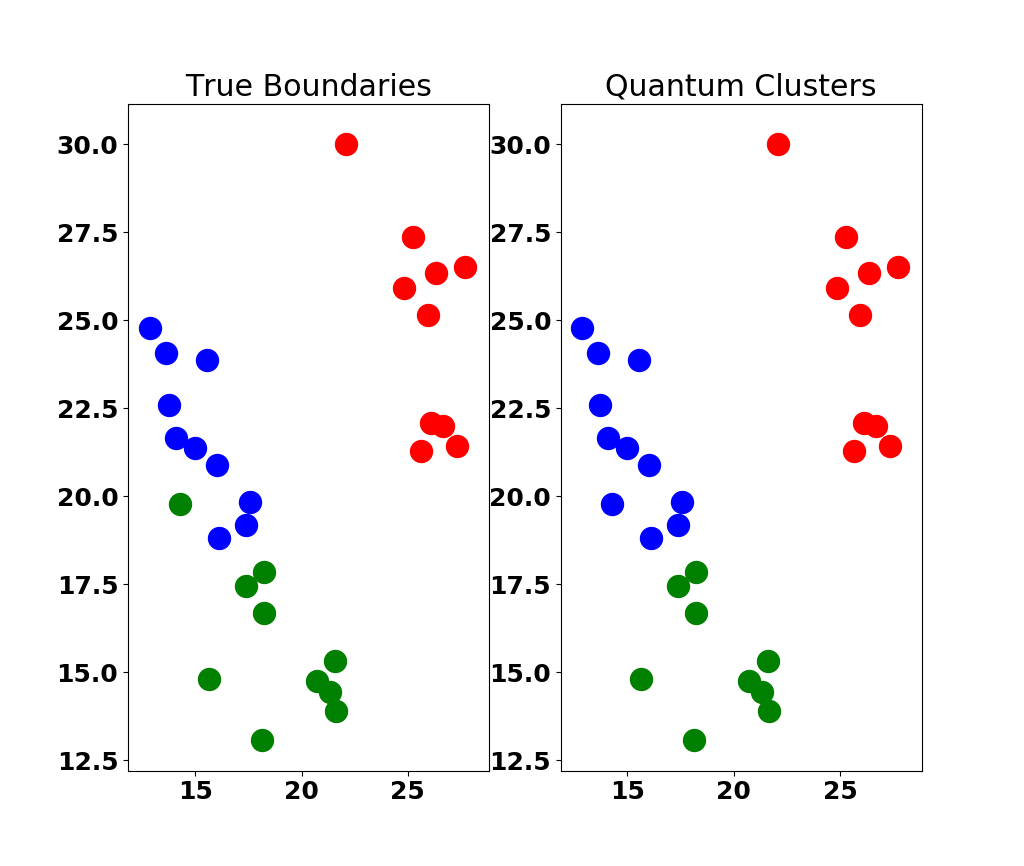
\includegraphics[height=7cm]{Figure_Wine1}
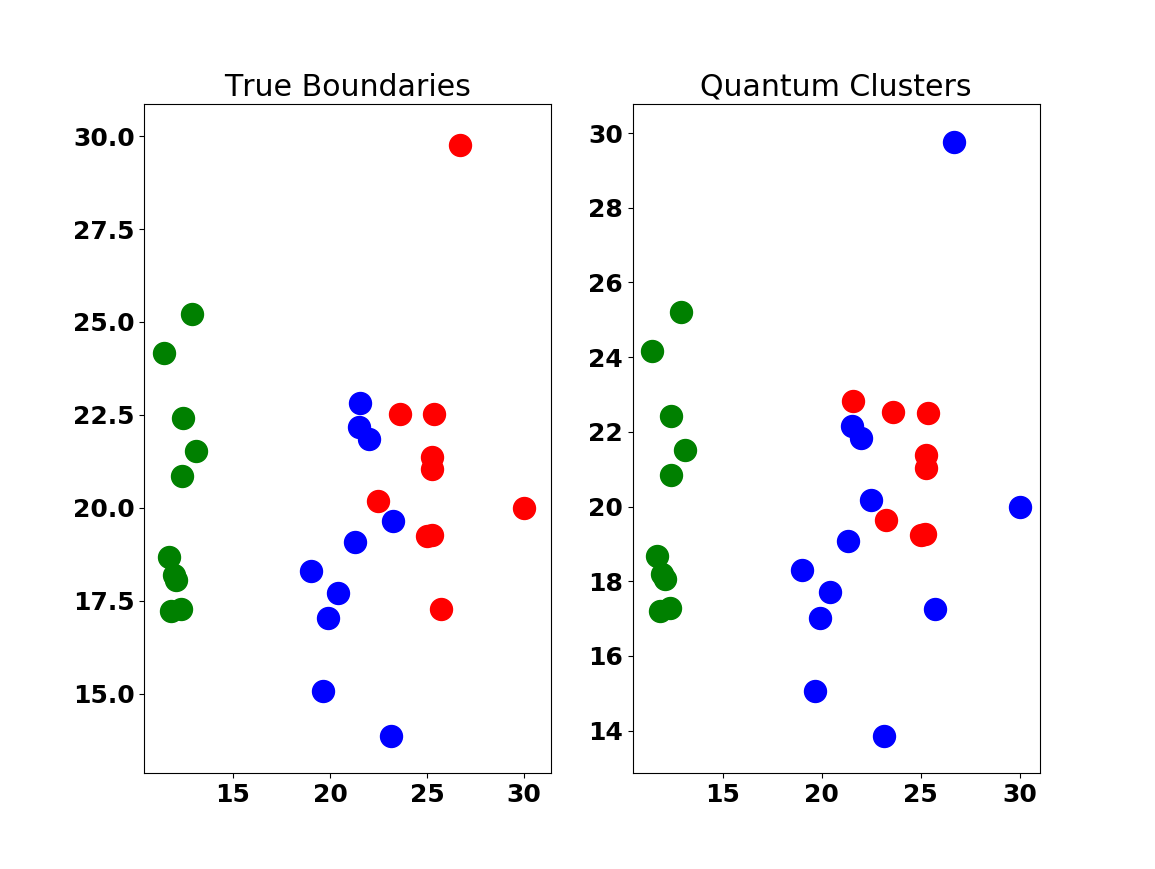
\includegraphics[height=7cm]{Figure_Iris1}
\caption{(Left) Wine dataset - True and predicted classifications with Quantum K-means algorithm. Predicted clusters almost exactly reflect true boundaries in the data - only one datapoint which lies near the boundary between two clusters is misclassified. The natural clustering in the Wine dataset is very accurately detected by our algorithm, showing that it tends to detect clustering at a level comparable to similar classical algorithms.}
\caption{(Right) Iris dataset - True and predicted classifications with Quantum K-means algorithm. Two of the three predicted clusters stray significantly from the true data boundaries. This is because there is little natural cluster separation between the two classes represented on the right side of the graphs, and as such, clustering algorithms do not perform well at classifying the data.}
\end{figure*}

\begin{table*}
\begin{tabular}{l|r|r}
&Accuracy&Time (s)\\
\hline
Classical SVM&96.7\%&0.0109\\
\cline{2-3}
&96.7\%&0.0031\\
\cline{2-3}
&96.7\%&0.0058\\
\cline{2-3}
&96.7\%&0.0029\\
\cline{2-3}
&96.7\%&0.0034\\
\hline\hline
Average&96.7\%&0.0052\\
\hline\hline
Quantum SVM by Havlicek et al.&63.3\%&103.9\\
\cline{2-3}
&63.3\%&105.4\\
\cline{2-3}
&63.3\%&106.5\\
\cline{2-3}
&63.3\%&103.4\\
\cline{2-3}
&63.3\%&104.2\\
\hline\hline
Average&63.3\%&104.7\\
\hline\hline
Classical K-means&70.0\%&0.0183\\
\cline{2-3}
&93.3\%&0.0139\\
\cline{2-3}
&90.0\%&0.0185\\
\cline{2-3}
&90.0\%&0.0141\\
\cline{2-3}
&100.0\%&0.0204\\
\hline\hline
Average&88.7\%&0.0170\\
\hline\hline
Quantum K-means&100.0\%&88.63\\
\cline{2-3}
&93.3\%&134.1\\
\cline{2-3}
&100.0\%&131.3\\
\cline{2-3}
&93.3\%&109.7\\
\cline{2-3}
&96.7\%&110.9\\
\hline\hline
Average&96.7\%&114.9\\
\hline\hline
\end{tabular}
\begin{tabular}{|l|r|r}
&Accuracy&Time (s)\\
\hline
Classical SVM&93.3\%&0.0070\\
\cline{2-3}
&93.3\%&0.0054\\
\cline{2-3}
&93.3\%&0.0061\\
\cline{2-3}
&93.3\%&0.0067\\
\cline{2-3}
&93.3\%&0.0066\\
\hline\hline
Average&93.3\%&0.0064\\
\hline\hline
Quantum SVM by Havlicek et al.&80.0\%&91.51\\
\cline{2-3}
&80.0\%&89.82\\
\cline{2-3}
&80.0\%&89.79\\
\cline{2-3}
&80.0\%&86.94\\
\cline{2-3}
&80.0\%&88.97\\
\hline\hline
Average&80.0\%&89.41\\
\hline\hline
Classical K-means&50.0\%&0.0044\\
\cline{2-3}
&86.7\%&0.0051\\
\cline{2-3}
&53.3\%&0.0083\\
\cline{2-3}
&86.7\%&0.0033\\
\cline{2-3}
&86.7\%&0.0083\\
\hline\hline
Average&72.7\%&0.0059\\
\hline\hline
Quantum K-means&70.0\%&108.6\\
\cline{2-3}
&73.3\%&107.9\\
\cline{2-3}
&76.7\%&110.5\\
\cline{2-3}
&80.0\%&102.5\\
\cline{2-3}
&76.7\%&108.9\\
\hline\hline
Average&75.3\%&107.7\\
\hline\hline
\end{tabular}
\caption{(Left) Trinary Classification on Wine Dataset. Each row depicts one trial, with the average of all 5 trials for each algorithm being shown at the bottom. As the Wine dataset contains natural clustering, both classical and quantum K-means clustering algorithms perform very well at classifying the data. Surprisingly, the quantum clustering algorithm performs better than its classical analogue. The quantum clustering algorithm converges in between 4-7 iterations. }
\caption{(Right) Trinary Classification on Iris Dataset. Each row depicts one trial, with the average of all 5 trials for each algorithm being shown at the bottom. As the Iris dataset does not contain much natural clustering, both classical and quantum K-means clustering algorithms suffer in performance at classifying the data. Still, the quantum clustering algorithm performs better than its classical analogue. The quantum clustering algorithm has trouble converging on the Iris dataset due to the cluster centroids being located very close together, which can cause problems due to uncertainty in the distance measure. As such, we force the algorithm to terminate after 6 iterations to get the data above.}
\end{table*}

\section{Trinary Classification}
Here, we apply our hybrid algorithm to real datasets. In order to get some idea of "accuracy", we use data with real class boundaries that we have access to, in order to compare our results to the true class separations. We also include the quantum SVM developed by Havlicek et. al in \cite{qsvm} for the sake of comparison. While \textit{K}-means clustering and the support vector machine belong to different classes of machine learning algorithms, with the former being a clustering algorithm and the latter being a supervised binary classification algorithm, we can compare them under certain constraints. We consider a trinary classification problem on the standard Wine and Iris datasets provided by the \textit{Scikit} module for machine learning on Python. For the \textit{K}-means clustering algorithms, we input the unlabeled test data and then compare the generated clusters with the true labels of the data. Then, we calculate the accuracy by calculating the percentage of correctly classified features. For the Support Vector Machine, we utilize the \textit{One Against Rest} multiclass extension provided by \textit{Qiskit} to extend the SVM to more than two classes. The \textit{One Against Rest} extension constructs a number of SVMs equal to the number of classes, each of which compare one class against all the others. See \cite{multiclass} for more details. We include a classical \textit{K}-means clustering algorithm as well as a classical RBF kernel SVM as controls. We run five experiments on each classifier, with 2 feature dimensions and 30 test inputs, as well as 30 training inputs for the SVMs. Note that the clustering algorithms are not provided with any training vectors and corresponding labels, while the SVMs are. All simulations were run with \textit{Qiskit Aer} on a Macbook Pro. Results of the simulations are shown in Table 1 and 2. Figure 1 and 2 graphically represent one run of the Quantum K-means algorithm on each dataset.

As expected, the SVM algorithms are much more consistent in terms of time and accuracy than the clustering methods. This is because the SVM is a supervised algorithm, and the amount of time that the clustering algorithm takes depends on how many iterations it must undergo, which consequently depends on the random initial seeding of the clusters. Surprisingly, the quantum \textit{K}-means clustering algorithm is more accurate than its classical counterpart on both datasets. The quantum \textit{K}-means algorithm takes several orders of magnitude more time to execute than its classical counterpart, but this is a consequence of simulating the quantum circuits as opposed to running them on a real machine. In general, as the dimension and size of the data increases, we strongly suspect that the hybrid algorithm will become less computationally expensive than the classical one to implement. We base this assertion off previous time complexity analysis done by Lloyd et al. \cite{lloydlearning} and Kerenidis et al. \cite{qmeans}. Additionally, it is well known that \textit{K}-means clustering algorithms are much less computationally expensive than SVMs on average, and we suspect that this holds for the quantum analogues of each algorithm (INSERT CITATION). We find that the clustering algorithms are much more successful in classifying the Wine dataset than the Iris dataset, which is to be expected as the Wine dataset possesses natural clustering between all of its classes while the Iris dataset does not. 

\section{Conclusions}
In this paper we introduced a hybrid algorithm for \textit{K}-means clustering, based on Lloyd's Algorithm and a novel technique of computation of Euclidean distance with quantum states. We find that the algorithm is successful in detecting natural clustering patterns in real data, and can reduce computation time of distance for large feature dimensions and many feature vectors when ran on a superconducting processor. This suggests that when one reasonably suspects there to be clustering in a large dataset, our algorithm can be useful in quickly finding those clusters for various data analysis uses. As described in \cite{lloydlearning}, there exists a purely adiabatic analogue to our hybrid algorithm which can save even more computational time in which cluster classification is conducted by perturbating a single quantum state which can then be sampled to return the clustering assignments with high probability. In the future we intend to attempt to construct and test such a clustering algorithm experimentally on an adiabatic quantum computer such as D-Wave.

\onecolumngrid
\bibliography{bibliography}{}
\end{document}